\subsection{Front-end}

\par Vue.js implementa il pattern architetturale MVVM (Model-View-ViewModel), una declinazione del pattern Model-View-Controller (MVC). In Vue 3, l’MVVM viene utilizzato implicitamente attraverso il modo in cui Vue gestisce i dati, la logica e l'interfaccia utente. Il ViewModel è un oggetto che sincronizza il Model e la View. Ogni istanza di Vue è un ViewModel.

\begin{figure}[H]
  \centering
  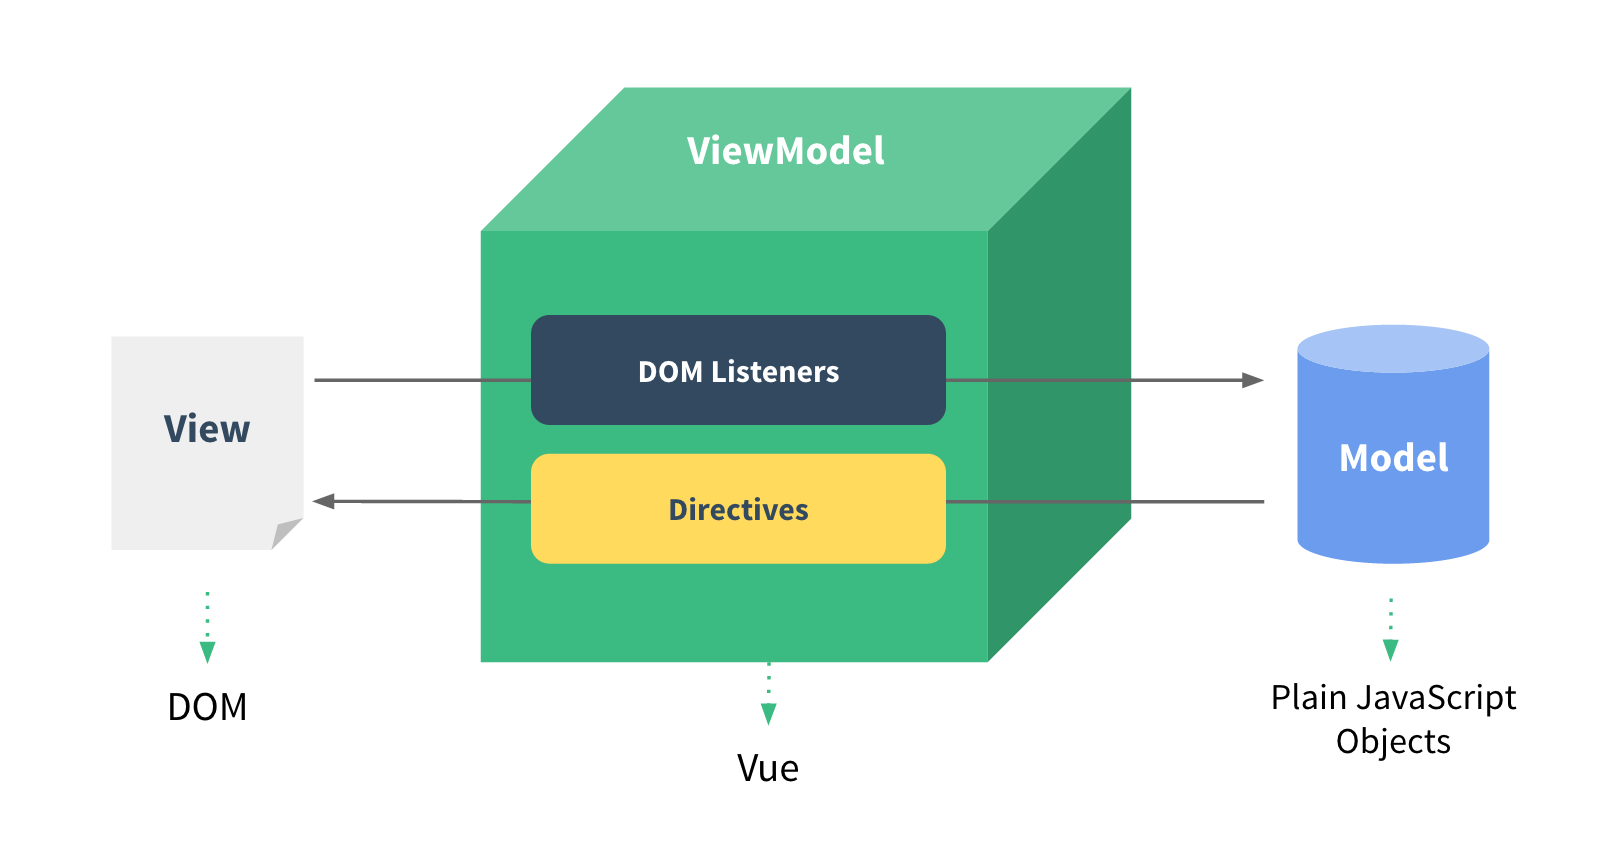
\includegraphics[width=0.95\textwidth]{assets/Frontend/architettura_mvvm.png}
  \caption{Model-View-ViewModel (MVVM)}
\end{figure}

\par Il pattern MVVM comprende tre layer, ciascuno con un ruolo specifico:
\begin{itemize}
  \item \textbf{Model}: è responsabile della gestione dei dati e della logica di business. In Vue.js, il Model è tipicamente rappresentato da semplici oggetti JavaScript (plain JavaScript objects) o data model objects (oggetti più strutturati) che diventano reattivi quando utilizzati dalle istanze di Vue. Inoltre, Vue offre soluzioni per la gestione centralizzata dello stato, come Vuex e Pinia;
  \item \textbf{View} (Presentation layer): è responsabile della presentazione dei dati all'utente. Descrive la struttura del DOM (Document Object Model). In Vue.js, la View è rappresentata dal template, che utilizza una sintassi HTML arricchita con binding e direttive specifiche per riflettere i cambiamento di stato. L'interfaccia viene aggiornata dinamicamente quando cambiano i dati del modello.
  \item \textbf{ViewModel}: è il layer che collega il Model e la View. Ha il compito di gestire le interazioni dell'utente e sincronizzare i dati con la View. Ogni istanza di Vue è un ViewModel. Oltre a sincronizzare il Model e la View, il ViewModel deve garantire una chiara separazione tra i dati e la logica di presentazione.
\end{itemize} 

\begin{figure}[H]
  \centering
  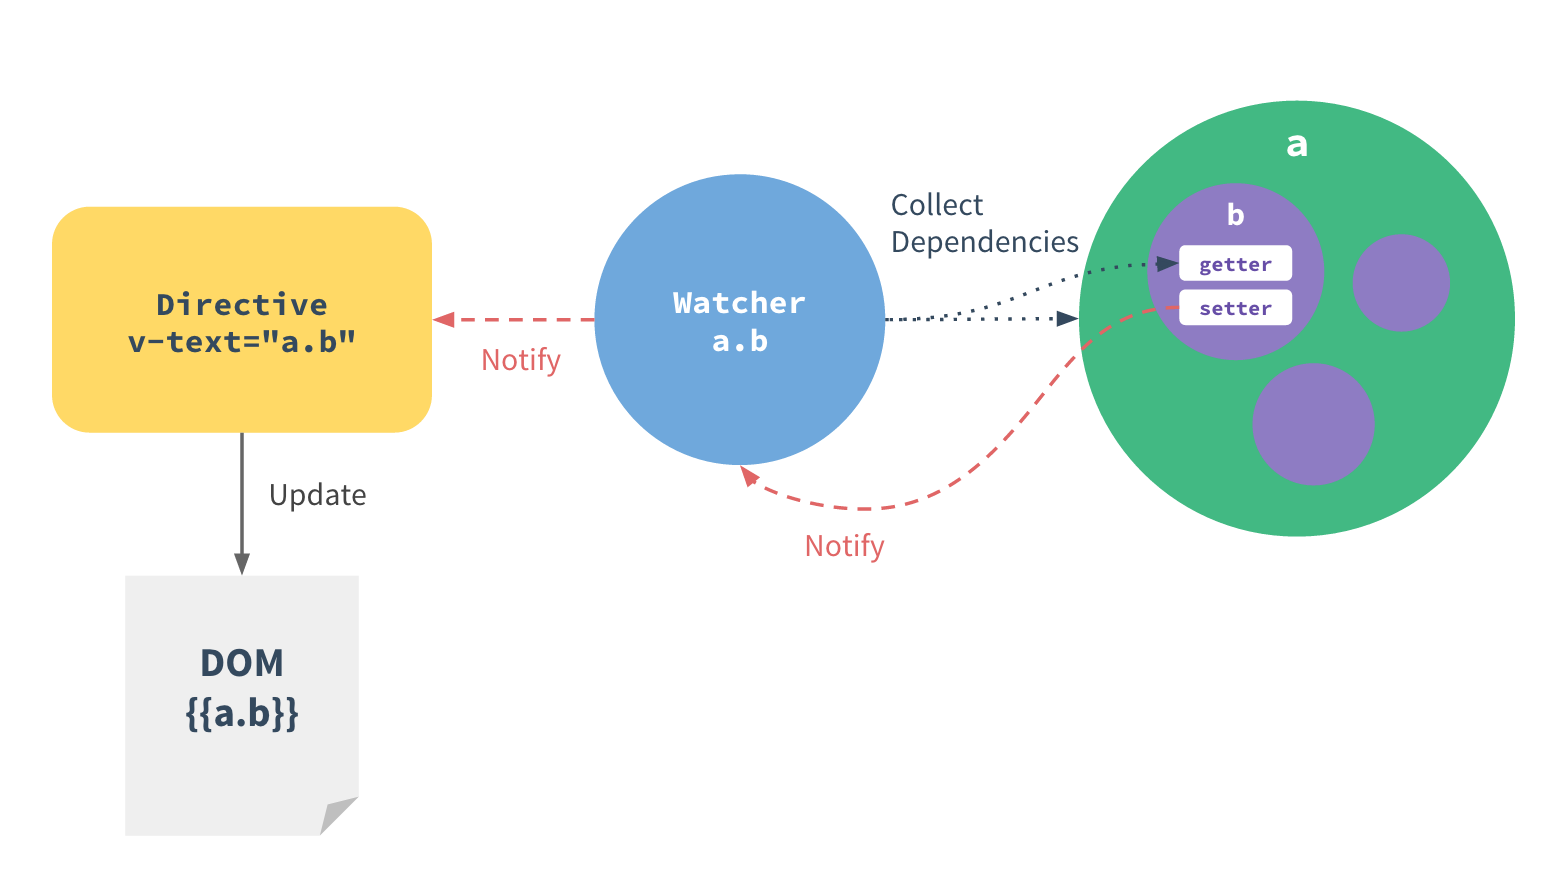
\includegraphics[width=0.95\textwidth]{assets/Frontend/overview_mvvm.png}
  \caption{Funzionamento del pattern MVVM}
\end{figure}

\par Vue.js implementa due concetti fondamentali:
\begin{itemize}
  \item \textbf{Reattività}: la reattività è un meccanismo che permette di aggiornare dinamicamente la View quando cambiano i dati del Model. I dati reattivi sono oggetti che vengono osservati da Vue. La differenza rispetto ai normali oggetti JavaScript è che Vue è in grado di intercettare l'accesso e la modifica di tutte le proprietà di un oggetto reattivo;
  \item \textbf{Composition API}: permette di suddividere la logica di un componente in funzioni riutilizzabili. La Composition API migliora la riusabilità, l'organizzazione e la manutenibilità del codice. Inoltre, le Composition API risolvono alcune limitazioni delle Options API, che emergono quando la logica di un singolo componente supera una determinata soglia di complessità.
\end{itemize}

\section{Progettazione dei componenti}

\subsection{Back-end}

%SEZIONE ROUTES DI dictionaries_api

\subsubsection{get\_all\_dictionaries}

\subsubsubsection{Descrizione}
\par La funzione \texttt{get\_all\_dictionaries} recupera tutti i dizionari presenti nel sistema e restituisce una risposta strutturata.

\subsubsubsection{Dettagli dell'endpoint}
\begin{itemize}
  \item \textbf{HTTP Method}: \texttt{GET};
  \item \textbf{Endpoint}: \texttt{/};
  \item \textbf{Tags}: \texttt{[tag]};
  \item \textbf{Response Model}: \texttt{DictionariesResponseDto};
  \item \textbf{Nome}: \texttt{getAllDictionaries};
  \item \textbf{Dependency Injection}:
  \begin{itemize}
    \item \textbf{dictionary\_service (DictionaryService)}: dipendenza risolta tramite Depends(get\_dictionary\_service).
  \end{itemize}
\end{itemize}

\subsubsubsection{Implementazione}
\begin{itemize}
  \item Effettua una chiamata al servizio di gestione dei dizionari per recuperare l'elenco completo dei dizionari;
  \item Restituisce un oggetto \texttt{DictionariesResponseDto} con lo stato della risposta e, in caso di successo, i dati richiesti.
\end{itemize}

\subsubsection{get\_dictionary}

\subsubsubsection{Descrizione}
\par La funzione \texttt{get\_dictionary} recupera un dizionario specifico utilizzando l'ID fornito e restituisce una risposta strutturata.

\subsubsubsection{Dettagli dell'endpoint}
\begin{itemize}
  \item \textbf{HTTP Method}: \texttt{GET};
  \item \textbf{Endpoint}: \texttt{/\{id\}/file};
  \item \textbf{Tags}: \texttt{[tag]};
  \item \textbf{Response Model}: \texttt{DictionaryResponseDto};
  \item \textbf{Nome}: \texttt{getDictionary};
  \item \textbf{Dependency Injection}:
  \begin{itemize}
    \item \textbf{dictionary\_service (DictionaryService)}: dipendenza risolta tramite Depends(get\_dictionary\_service).
  \end{itemize}
  \item \textbf{Parametri}:
  \begin{itemize}
    \item \textbf{id (int)}: ID del dizionario da recuperare.
  \end{itemize}
\end{itemize}

\subsubsubsection{Implementazione}
\begin{itemize}
  \item Effettua una chiamata al servizio di gestione dei dizionari per recuperare i dettagli di un dizionario specifico;
  \item Restituisce un oggetto \texttt{DictionaryResponseDto} con lo stato della risposta e, in caso di successo, i dati richiesti.
\end{itemize}

\subsubsection{get\_dictionary\_file}

\subsubsubsection{Descrizione}
\par La funzione \texttt{get\_dictionary\_file} recupera un file di dizionario specifico dal database utilizzando l'ID fornito e restituisce una risposta strutturata.

\subsubsubsection{Dettagli dell'Endpoint}
\begin{itemize}
\item \textbf{HTTP Method}: \texttt{GET};
\item \textbf{Endpoint}: \texttt{/\{id\}/file};
\item \textbf{Tags}: \texttt{[tag]};
\item \textbf{Nome}: \texttt{getDictionaryFile};
\item \textbf{Dependency Injection}:
\begin{itemize}
\item \textbf{db (Session)}: Dipendenza risolta tramite \texttt{Depends(get\_db)}.
\end{itemize}
\item \textbf{Parametri}:
\begin{itemize}
\item \textbf{id (int)}: ID del dizionario di cui recuperare il file.
\end{itemize}
\end{itemize}

\subsubsubsection{Implementazione}
\begin{itemize}
\item Recupera il dizionario dal database utilizzando \texttt{crud.get\_dictionary\_by\_id(db, id)};
\item Se il dizionario viene trovato, restituisce un \texttt{FileResponse} con il nome del file generato tramite \texttt{\_\_generate\_schema\_file\_name(id)};
\item Se il dizionario non viene trovato, restituisce un oggetto \texttt{ResponseDto} con un messaggio di errore e lo stato \texttt{ResponseStatusEnum.NOT\_FOUND}.
\end{itemize}

\subsubsection{get\_dictionary\_preview}

\subsubsubsection{Descrizione}
\par La funzione \texttt{get\_dictionary\_preview} recupera un'anteprima di un dizionario specifico dal database utilizzando l'ID fornito e restituisce una risposta strutturata.

\subsubsubsection{Dettagli dell'Endpoint}
\begin{itemize}
\item \textbf{HTTP Method}: \texttt{GET};
\item \textbf{Endpoint}: \texttt{/\{id\}/dictionary-preview};
\item \textbf{Tags}: \texttt{[tag]};
\item \textbf{Response Model}: \texttt{DictionaryResponseDto};
\item \textbf{Nome}: \texttt{getDictionaryPreview};
\item \textbf{Dependency Injection}:
\begin{itemize}
\item \textbf{db (Session)}: Dipendenza risolta tramite \texttt{Depends(get\_db)}.
\end{itemize}
\item \textbf{Parametri}:
\begin{itemize}
\item \textbf{id (int)}: ID del dizionario di cui recuperare l'anteprima.
\end{itemize}
\end{itemize}

\subsubsubsection{Implementazione}
\begin{itemize}
\item Recupera il dizionario dal database utilizzando \texttt{crud.get\_dictionary\_by\_id(db, id)}.
\item Se il dizionario viene trovato:
\begin{itemize}
\item Estrae un sotto-schema del dizionario utilizzando \texttt{SchemaMultiExtractor\-.\-extract\_preview(id)};
\item Crea un oggetto \texttt{DictionaryPreviewDto} con i dettagli del sotto-schema;
\item Restituisce un oggetto \texttt{DictionaryResponseDto} con i dati dell'anteprima del dizionario e lo stato \texttt{ResponseStatusEnum.OK};
\end{itemize}
\item Se il dizionario non viene trovato, restituisce un oggetto \texttt{ResponseDto} con un messaggio di errore e lo stato \texttt{ResponseStatusEnum.NOT\_FOUND}.
\end{itemize}

\subsubsection{create\_dictionary}

\subsubsubsection{Descrizione}
\par La funzione \texttt{create\_dictionary} permette di creare un nuovo dizionario nel database utilizzando i dati forniti e un file di schema. La funzione include controlli di validità e verifica l'unicità del nome del dizionario.

\subsubsubsection{Dettagli dell'Endpoint}
\begin{itemize}
\item \textbf{HTTP Method}: \texttt{POST};
\item \textbf{Endpoint}: \texttt{/};
\item \textbf{Tags}: \texttt{[tag]};
\item \textbf{Response Model}: \texttt{DictionaryResponseDto};
\item \textbf{Dependencies}:
\begin{itemize}
\item \texttt{Depends(JwtBearer())}: Assicura che l'endpoint sia protetto da un meccanismo di autenticazione JWT.
\end{itemize}
\item \textbf{Nome}: \texttt{createDictionary};
\item \textbf{Dependency Injection}:
\begin{itemize}
\item \textbf{file (Annotated[UploadFile, File()])}: Il file di schema del dizionario da caricare;
\item \textbf{dictionary (DictionaryDto)}: I dati del dizionario, ottenuti tramite \texttt{Depends()};
\item \textbf{db (Session)}: Dipendenza risolta tramite \texttt{Depends(get\_db)}.
\end{itemize}
\end{itemize}

\subsubsubsection{Implementazione}
\begin{itemize}
\item Verifica che il nome e la descrizione del dizionario, oltre al file, siano presenti;
\item Recupera un dizionario esistente con lo stesso nome utilizzando \texttt{crud.get\_\-dictionary\-\_by\_name(db, name=dictionary.name)};
\item Se il dizionario esiste già, restituisce un oggetto \texttt{DictionaryResponseDto} con \texttt{data\-=\-None}, un messaggio di errore e lo stato \texttt{ResponseStatusEnum.CONFLICT};
\item Crea un nuovo dizionario utilizzando \texttt{crud.create\_dictionary(db=db, dictionary\-=\-dictionary)};
\item Legge il contenuto del file e valida il formato dello schema del dizionario utilizzando \texttt{DictionaryValidator.validate(Utils.string\_to\_json(content))};
\item Se lo schema non è valido, restituisce un oggetto \texttt{DictionaryResponseDto} con \texttt{data=None}, un messaggio di errore e lo stato \texttt{ResponseStatusEnum.BAD\_REQUEST};
\item Scrive il contenuto del file in un nuovo file utilizzando \texttt{aiofiles.open(\_\_generate\-\_\-schema\-\_file\-\_name(new\_dic.id), "wb")};
\item Crea un indice \texttt{txtai} utilizzando \texttt{manager.create\_index(new\_dic.id)};
\item Restituisce un oggetto \texttt{DictionaryResponseDto} con i dati del nuovo dizionario e lo stato \texttt{ResponseStatusEnum.OK};
\item Se il file non è presente, restituisce un oggetto \texttt{DictionaryResponseDto} con \texttt{data=None}, un messaggio di errore e lo stato \texttt{ResponseStatusEnum.BAD\_REQUEST};
\item Se il nome e la descrizione del dizionario non sono presenti, restituisce un oggetto \texttt{DictionaryResponseDto} con \texttt{data=None}, un messaggio di errore e lo stato \texttt{ResponseStatusEnum.BAD\_REQUEST}.
\end{itemize}

\subsubsection{update\_dictionary\_file}

\subsubsubsection{Descrizione}
\par La funzione \texttt{update\_dictionary\_file} permette di aggiornare il file di schema di un dizionario esistente nel database utilizzando l'ID fornito e un nuovo file di schema. La funzione include controlli di validità dello schema.

\subsubsubsection{Dettagli dell'Endpoint}
\begin{itemize}
\item \textbf{HTTP Method}: \texttt{PUT};
\item \textbf{Endpoint}: \texttt{/\{id\}/file};
\item \textbf{Tags}: \texttt{[tag]};
\item \textbf{Response Model}: \texttt{DictionaryResponseDto};
\item \textbf{Dependencies}:
\begin{itemize}
\item \texttt{Depends(JwtBearer())}: Assicura che l'endpoint sia protetto da un meccanismo di autenticazione JWT.
\end{itemize}
\item \textbf{Nome}: \texttt{updateDictionaryFile};
\item \textbf{Dependency Injection}:
\begin{itemize}
\item \textbf{file (Annotated[UploadFile, File()])}: Il nuovo file di schema del dizionario da caricare;
\item \textbf{db (Session)}: Dipendenza risolta tramite \texttt{Depends(get\_db)}.
\end{itemize}
\item \textbf{Parametri}:
\begin{itemize}
\item \textbf{id (int)}: ID del dizionario di cui aggiornare il file.
\end{itemize}
\end{itemize}

\subsubsubsection{Implementazione}
\begin{itemize}
\item Recupera il dizionario dal database utilizzando \texttt{crud.get\_dictionary\_by\_id(db, id)};
\item Se il dizionario non viene trovato, restituisce un oggetto \texttt{DictionaryResponseDto} con \texttt{data=None}, un messaggio di errore e lo stato \texttt{ResponseStatusEnum.NOT\_FOUND};
\item Legge il contenuto del file e valida il formato dello schema del dizionario utilizzando \texttt{DictionaryValidator.validate(Utils.string\_to\_json(content))};
\item Se lo schema non è valido, restituisce un oggetto \texttt{DictionaryResponseDto} con \texttt{data=None}, un messaggio di errore e lo stato \texttt{ResponseStatusEnum.BAD\_REQUEST};
\item Scrive il contenuto del file in un nuovo file utilizzando \texttt{aiofiles.open(\_\_generate\_s\-chema\_file\_name(id), "wb")};
\item Aggiorna l'indice \texttt{txtai} utilizzando \texttt{manager.create\_index(found\_dic.id)};
\item Restituisce un oggetto \texttt{DictionaryResponseDto} con i dati del dizionario aggiornato e lo stato \texttt{ResponseStatusEnum.OK}.
\end{itemize}

\subsubsection{update\_dictionary\_metadata}

\subsubsubsection{Descrizione}
\par La funzione \texttt{update\_dictionary\_metadata} permette di aggiornare i metadati di un dizionario esistente nel database utilizzando l'ID fornito e un oggetto \texttt{DictionaryDto}. La funzione include controlli di validità e verifica l'unicità del nome del dizionario.

\subsubsubsection{Dettagli dell'Endpoint}
\begin{itemize}
\item \textbf{HTTP Method}: \texttt{PUT};
\item \textbf{Endpoint}: \texttt{/\{id\}};
\item \textbf{Tags}: \texttt{[tag]};
\item \textbf{Response Model}: \texttt{DictionaryResponseDto};
\item \textbf{Dependencies}:
\begin{itemize}
\item \texttt{Depends(JwtBearer())}: Assicura che l'endpoint sia protetto da un meccanismo di autenticazione JWT.
\end{itemize}
\item \textbf{Nome}: \texttt{updateDictionaryMetadata};
\item \textbf{Dependency Injection}:
\begin{itemize}
\item \textbf{dictionary (DictionaryDto)}: I nuovi metadati del dizionario;
\item \textbf{db (Session)}: Dipendenza risolta tramite \texttt{Depends(get\_db)}.
\end{itemize}
\item \textbf{Parametri}:
\begin{itemize}
\item \textbf{id (int)}: ID del dizionario di cui aggiornare i metadati.
\end{itemize}
\end{itemize}

\subsubsubsection{Implementazione}
\begin{itemize}
\item Recupera il dizionario dal database utilizzando \texttt{crud.get\_dictionary\_by\_id(db, id)};
\item Se il dizionario non viene trovato, restituisce un oggetto \texttt{DictionaryResponseDto} con \texttt{data=None}, un messaggio di errore e lo stato \texttt{ResponseStatusEnum.NOT\_FOUND};
\item Se il nome o la descrizione del dizionario sono assenti, restituisce un oggetto \texttt{DictionaryResponseDto} con \texttt{data=None}, un messaggio di errore e lo stato \texttt{Response\-StatusEnum.BAD\_REQUEST};
\item Verifica se esiste un altro dizionario con lo stesso nome utilizzando \texttt{crud.get\-\_\-dictionary\-\_by\_name(db, dictionary.name)};
\item Se esiste un altro dizionario con lo stesso nome e l'ID è diverso, restituisce un oggetto \texttt{DictionaryResponseDto} con \texttt{data=None}, un messaggio di errore e lo stato \texttt{ResponseStatusEnum.CONFLICT};
\item Aggiorna il dizionario utilizzando \texttt{crud.update\_dictionary(db, dictionary)};
\item Restituisce un oggetto \texttt{DictionaryResponseDto} con i dati del dizionario aggiornato e lo stato \texttt{ResponseStatusEnum.OK}.
\end{itemize}

\subsubsection{delete\_dictionary}

\subsubsubsection{Descrizione}
\par La funzione \texttt{delete\_dictionary} permette di eliminare un dizionario esistente dal database utilizzando l'ID fornito. La funzione elimina anche il file di schema associato e l'indice \texttt{txtai}.

\subsubsubsection{Dettagli dell'Endpoint}
\begin{itemize}
\item \textbf{HTTP Method}: \texttt{DELETE};
\item \textbf{Endpoint}: \texttt{/\{id\}};
\item \textbf{Tags}: \texttt{[tag]};
\item \textbf{Response Model}: \texttt{ResponseDto};
\item \textbf{Nome}: \texttt{deleteDictionary};
\item \textbf{Dependency Injection}:
\begin{itemize}
\item \textbf{db (Session)}: Dipendenza risolta tramite \texttt{Depends(get\_db)}.
\end{itemize}
\item \textbf{Parametri}:
\begin{itemize}
\item \textbf{id (int)}: ID del dizionario da eliminare.
\end{itemize}
\end{itemize}

\subsubsubsection{Implementazione}
\begin{itemize}
\item Recupera il dizionario dal database utilizzando \texttt{crud.get\_dictionary\_by\_id(db, id)};
\item Se il dizionario non viene trovato, restituisce un oggetto \texttt{ResponseDto} con un messaggio di errore e lo stato \texttt{ResponseStatusEnum.NOT\_FOUND};
\item Elimina il dizionario dal database utilizzando \texttt{crud.delete\_dictionary(db, id)};
\item Se il file di schema esiste, lo elimina utilizzando \texttt{os.remove(\_\_generate\_schema\-\_\-file\_name(id))};
\item Elimina l'indice \texttt{txtai} utilizzando \texttt{manager.delete\_index(found\_dic.id)};
\item Restituisce un oggetto \texttt{ResponseDto} con lo stato \texttt{ResponseStatusEnum.OK}.
\end{itemize}

%SEZIONE ROUTES DI login_api

\subsubsection{login}

\subsubsubsection{Descrizione}
\par La funzione \texttt{login} permette di autenticare un utente utilizzando le credenziali fornite. Se le credenziali sono corrette, viene restituito un token JWT.

\subsubsubsection{Dettagli dell'Endpoint}
\begin{itemize}
\item \textbf{HTTP Method}: \texttt{POST};
\item \textbf{Endpoint}: \texttt{/};
\item \textbf{Tags}: \texttt{[tag]};
\item \textbf{Response Model}: \texttt{AuthResponseDto};
\item \textbf{Nome}: \texttt{login};
\item \textbf{Dependency Injection}:
\begin{itemize}
\item \textbf{data (LoginDto)}: I dati di login dell'utente;
\item \textbf{db (Session)}: Dipendenza risolta tramite \texttt{Depends(get\_db)}.
\end{itemize}
\end{itemize}

\subsubsubsection{Implementazione}
\begin{itemize}
\item Recupera l'utente dal database utilizzando \texttt{crud.get\_user\_by\_username(db,\- data\-.username)};
\item Se l'utente non viene trovato, restituisce un oggetto \texttt{AuthResponseDto} con \texttt{data\-=\-None} e lo stato \texttt{ResponseStatusEnum.NOT\_FOUND};
\item Se la password non è corretta, restituisce un oggetto \texttt{AuthResponseDto} con \texttt{data\-=\-None}, un messaggio di errore e lo stato \texttt{ResponseStatusEnum.BAD\_CREDENTIAL};
\item Genera un token JWT utilizzando \texttt{JwtHandler.sign(query.id)};
\item Restituisce un oggetto \texttt{AuthResponseDto} con il token generato e lo stato \texttt{Response\-Status\-Enum.OK}.
\end{itemize}

%SEZIONE ROUTES DI prompt_api

\subsubsection{generate\_prompt}

\subsubsubsection{Descrizione}
\par La funzione \texttt{generate\_prompt} genera un prompt utilizzando i parametri forniti dall'utente, tra cui un dizionario specifico, una query, il DBMS e la lingua.

\subsubsubsection{Dettagli dell'Endpoint}
\begin{itemize}
\item \textbf{HTTP Method}: \texttt{GET};
\item \textbf{Endpoint}: \texttt{/};
\item \textbf{Tags}: \texttt{[tag]};
\item \textbf{Response Model}: \texttt{StringDataResponseDto};
\item \textbf{Nome}: \texttt{generatePrompt};
\item \textbf{Dependency Injection}:
\begin{itemize}
\item \textbf{dictionary\_id (Annotated[int, Query(alias="dictionaryId")])}: L'ID del dizionario da utilizzare;
\item \textbf{query (str)}: La query fornita dall'utente;
\item \textbf{dbms (str)}: Il sistema di gestione del database (DBMS);
\item \textbf{lang (str)}: La lingua da utilizzare;
\item \textbf{prompt\_manager\_service (PromptManagerService)}: Dipendenza risolta tramite \texttt{Depends(get\_prompt\_manager\_service)}.
\end{itemize}
\end{itemize}

\subsubsubsection{Implementazione}
\begin{itemize}
\item Genera il prompt basato sui parametri forniti (dizionario, query, lingua, DBMS);
\item Restituisce un oggetto \texttt{StringDataResponseDto} con il prompt generato.
\end{itemize}

\subsubsection{generate\_prompt\_with\_debug}

\subsubsubsection{Descrizione}
\par La funzione \texttt{generate\_prompt\_with\_debug} genera un prompt e include informazioni dettagliate di debug, fornendo dati aggiuntivi per la risoluzione di problemi.

\subsubsubsection{Dettagli dell'Endpoint}
\begin{itemize}
\item \textbf{HTTP Method}: \texttt{GET};
\item \textbf{Endpoint}: \texttt{/debug};
\item \textbf{Tags}: \texttt{[tag]};
\item \textbf{Response Model}: \texttt{PromptResponseDto};
\item \textbf{Nome}: \texttt{generatePromptWithDebug};
\item \textbf{Dependency Injection}:
\begin{itemize}
\item \textbf{dictionary\_id (Annotated[int, Query(alias="dictionaryId")])}: L'ID del dizionario da utilizzare;
\item \textbf{query (str)}: La query fornita dall'utente;
\item \textbf{dbms (str)}: Il sistema di gestione del database (DBMS);
\item \textbf{lang (str)}: La lingua da utilizzare;
\item \textbf{prompt\_manager\_service (PromptManagerService)}: Dipendenza risolta tramite \texttt{Depends(get\_prompt\_manager\_service)};
\item \textbf{JWT Authentication}: Autenticazione richiesta tramite \texttt{Depends(JwtBearer())}.
\end{itemize}
\end{itemize}

\subsubsubsection{Implementazione}
\begin{itemize}
\item Genera un prompt basato sui parametri forniti e include informazioni di debug;
\item Restituisce un oggetto \texttt{PromptResponseDto} con il prompt generato e i dati di debug.
\end{itemize}


% TABELLA TRACCIAMENTO REQUISITI

\subsubsection{Tracciamento dei requisiti}
\bgroup
\begin{adjustwidth}{-0.5cm}{-0.5cm}
	\centering
	% MAX 12.5cm
  \begin{longtable}{|c|c|}
		\caption{Tracciamento dei requisiti back-end}
  	\label{tab:tracciamento-requisiti-back-end} \\
    \hline
		\textbf{ID} & \textbf{Route} \\
		\hline
		\endfirsthead

		\caption[]{Tracciamento dei requisiti back-end (continua)} \\
		\hline
		\textbf{ID} & \textbf{Route} \\
		\hline
		\endhead

		\hline
		\multicolumn{2}{|r|}{{Continua nella prossima pagina}} \\
		\hline
		\endfoot

		\hline
		\endlastfoot

    RF.O.1 & \texttt{login} \\
	  \hline RF.O.2 & \texttt{login} \\
    \hline RF.O.3 & \texttt{generate\_prompt}\\
    \hline RF.O.6 & \texttt{generate\_prompt}, \texttt{generate\_prompt\_with\_debug} \\
    \hline RF.O.9 & \texttt{get\_all\_dictionaries} \\
    \hline RF.O.9.1 & \texttt{get\_all\_dictionaries} \\
    \hline RF.O.10 & \texttt{get\_all\_dictionaries}, \texttt{get\_dictionary} \\
    \hline RF.O.10.1 & \texttt{get\_all\_dictionaries}, \texttt{get\_dictionary} \\
    \hline RF.O.10.2 & \texttt{get\_all\_dictionaries}, \texttt{get\_dictionary} \\
    \hline RF.O.10.3 & \texttt{get\_all\_dictionaries}, \texttt{get\_dictionary} \\
    \hline RF.O.11 & \texttt{generate\_prompt}, \texttt{generate\_prompt\_with\_debug} \\
    \hline RF.O.13 & \texttt{create\_dictionary} \\
    \hline RF.O.14 & \texttt{get\_dictionary\_preview} \\
    \hline RF.O.14.1 & \texttt{get\_dictionary\_preview} \\
    \hline RF.O.14.2 & \texttt{get\_dictionary\_preview} \\
    \hline RF.O.14.3 & \texttt{get\_dictionary\_preview} \\
    \hline RF.O.14.3.1 & \texttt{get\_dictionary\_preview} \\
    \hline RF.O.14.3.1.1 & \texttt{get\_dictionary\_preview} \\
    \hline RF.O.14.3.1.2 & \texttt{get\_dictionary\_preview} \\
    \hline RF.O.15 & \texttt{create\_dictionary} \\
    \hline RF.O.16 & \texttt{create\_dictionary} \\
    \hline RF.O.17 & \texttt{create\_dictionary} \\
    \hline RF.O.18 & \texttt{delete\_dictionary} \\
    \hline RF.O.19 & \texttt{create\_dictionary}, \texttt{update\_dictionary\_file} \\
    \hline RF.O.20 & \texttt{update\_dictionary\_file} \\
    \hline RF.O.21 & \texttt{delete\_dictionary} \\
    \hline RF.O.22 & \texttt{generate\_prompt\_with\_debug} \\
    \hline RF.O.28 & \texttt{create\_dictionary}, \texttt{update\_dictionary\_file} \\
    \hline RF.O.29 & \texttt{update\_dictionary\_metadata} \\
    \hline RF.O.30 & \texttt{update\_dictionary\_metadata} \\
    \hline RF.O.31 & \texttt{create\_dictionary}, \texttt{update\_dictionary\_metadata} \\
    \hline RF.O.31.1 & \texttt{create\_dictionary}, \texttt{update\_dictionary\_metadata} \\
    \hline RF.O.31.2 & \texttt{create\_dictionary}, \texttt{update\_dictionary\_metadata} \\
    \hline RF.O.32 & \texttt{create\_dictionary}, \texttt{update\_dictionary\_metadata} \\
    \hline RF.O.33 & \texttt{create\_dictionary}, \texttt{update\_dictionary\_file} \\
    \hline RF.O.34 & \texttt{create\_dictionary}, \texttt{update\_dictionary\_file} \\
    \hline RF.O.35 & \texttt{generate\_prompt}, \texttt{generate\_prompt\_with\_debug} \\
    \hline RF.O.37 & \texttt{get\_dictionary\_file} \\
    \hline RF.O.39 & \texttt{create\_dictionary}, \texttt{update\_dictionary\_file} \\
    \hline RF.D.40 & \texttt{create\_dictionary}, \texttt{update\_dictionary\_file} \\
    \hline RF.O.41 & \texttt{generate\_prompt}, \texttt{generate\_prompt\_with\_debug} \\
    \hline RF.OP.42 & \texttt{generate\_prompt}, \texttt{generate\_prompt\_with\_debug} \\
    \hline RF.O.45 & \texttt{generate\_prompt}, \texttt{generate\_prompt\_with\_debug} \\
    \hline RF.O.46 & \texttt{generate\_prompt\_with\_debug} \\
    \hline RF.O.47 & \texttt{generate\_prompt}, \texttt{generate\_prompt\_with\_debug} \\
    \hline RF.D.52 & \texttt{generate\_prompt}, \texttt{generate\_prompt\_with\_debug} \\
    \hline RF.O.55 & \texttt{create\_dictionary}, \texttt{update\_dictionary\_file} \\
    \hline RF.O.56 & \texttt{create\_dictionary}, \texttt{update\_dictionary\_file} \\
    \hline RF.O.57 & \texttt{create\_dictionary}, \texttt{update\_dictionary\_file} \\
  \end{longtable}
\end{adjustwidth}
\egroup
\subsection{Back-end}

%SEZIONE ROUTES DI dictionaries_api

\subsubsection{get\_all\_dictionaries}

\subsubsubsection{Descrizione}
\par La funzione \texttt{get\_all\_dictionaries} recupera tutti i dizionari presenti nel sistema e restituisce una risposta strutturata.

\subsubsubsection{Dettagli dell'endpoint}
\begin{itemize}
  \item \textbf{HTTP Method}: \texttt{GET};
  \item \textbf{Endpoint}: \texttt{/};
  \item \textbf{Tags}: \texttt{[tag]};
  \item \textbf{Response Model}: \texttt{DictionariesResponseDto};
  \item \textbf{Nome}: \texttt{getAllDictionaries};
  \item \textbf{Dependency Injection}:
  \begin{itemize}
    \item \textbf{dictionary\_service (DictionaryService)}: dipendenza risolta tramite Depends(get\_dictionary\_service).
  \end{itemize}
\end{itemize}

\subsubsubsection{Implementazione}
\begin{itemize}
  \item Effettua una chiamata al servizio di gestione dei dizionari per recuperare l'elenco completo dei dizionari;
  \item Restituisce un oggetto \texttt{DictionariesResponseDto} con lo stato della risposta e, in caso di successo, i dati richiesti.
\end{itemize}

\subsubsection{get\_dictionary}

\subsubsubsection{Descrizione}
\par La funzione \texttt{get\_dictionary} recupera un dizionario specifico utilizzando l'ID fornito e restituisce una risposta strutturata.

\subsubsubsection{Dettagli dell'endpoint}
\begin{itemize}
  \item \textbf{HTTP Method}: \texttt{GET};
  \item \textbf{Endpoint}: \texttt{/\{id\}/file};
  \item \textbf{Tags}: \texttt{[tag]};
  \item \textbf{Response Model}: \texttt{DictionaryResponseDto};
  \item \textbf{Nome}: \texttt{getDictionary};
  \item \textbf{Dependency Injection}:
  \begin{itemize}
    \item \textbf{dictionary\_service (DictionaryService)}: dipendenza risolta tramite Depends(get\_dictionary\_service).
  \end{itemize}
  \item \textbf{Parametri}:
  \begin{itemize}
    \item \textbf{id (int)}: ID del dizionario da recuperare.
  \end{itemize}
\end{itemize}

\subsubsubsection{Implementazione}
\begin{itemize}
  \item Effettua una chiamata al servizio di gestione dei dizionari per recuperare i dettagli di un dizionario specifico;
  \item Restituisce un oggetto \texttt{DictionaryResponseDto} con lo stato della risposta e, in caso di successo, i dati richiesti.
\end{itemize}

\subsubsection{get\_dictionary\_file}

\subsubsubsection{Descrizione}
\par La funzione \texttt{get\_dictionary\_file} recupera un file di dizionario specifico dal database utilizzando l'ID fornito e restituisce una risposta strutturata.

\subsubsubsection{Dettagli dell'Endpoint}
\begin{itemize}
\item \textbf{HTTP Method}: \texttt{GET};
\item \textbf{Endpoint}: \texttt{/\{id\}/file};
\item \textbf{Tags}: \texttt{[tag]};
\item \textbf{Nome}: \texttt{getDictionaryFile};
\item \textbf{Dependency Injection}:
\begin{itemize}
\item \textbf{db (Session)}: Dipendenza risolta tramite \texttt{Depends(get\_db)}.
\end{itemize}
\item \textbf{Parametri}:
\begin{itemize}
\item \textbf{id (int)}: ID del dizionario di cui recuperare il file.
\end{itemize}
\end{itemize}

\subsubsubsection{Implementazione}
\begin{itemize}
\item Recupera il dizionario dal database utilizzando \texttt{crud.get\_dictionary\_by\_id(db, id)};
\item Se il dizionario viene trovato, restituisce un \texttt{FileResponse} con il nome del file generato tramite \texttt{\_\_generate\_schema\_file\_name(id)};
\item Se il dizionario non viene trovato, restituisce un oggetto \texttt{ResponseDto} con un messaggio di errore e lo stato \texttt{ResponseStatusEnum.NOT\_FOUND}.
\end{itemize}

\subsubsection{get\_dictionary\_preview}

\subsubsubsection{Descrizione}
\par La funzione \texttt{get\_dictionary\_preview} recupera un'anteprima di un dizionario specifico dal database utilizzando l'ID fornito e restituisce una risposta strutturata.

\subsubsubsection{Dettagli dell'Endpoint}
\begin{itemize}
\item \textbf{HTTP Method}: \texttt{GET};
\item \textbf{Endpoint}: \texttt{/\{id\}/dictionary-preview};
\item \textbf{Tags}: \texttt{[tag]};
\item \textbf{Response Model}: \texttt{DictionaryResponseDto};
\item \textbf{Nome}: \texttt{getDictionaryPreview};
\item \textbf{Dependency Injection}:
\begin{itemize}
\item \textbf{db (Session)}: Dipendenza risolta tramite \texttt{Depends(get\_db)}.
\end{itemize}
\item \textbf{Parametri}:
\begin{itemize}
\item \textbf{id (int)}: ID del dizionario di cui recuperare l'anteprima.
\end{itemize}
\end{itemize}

\subsubsubsection{Implementazione}
\begin{itemize}
\item Recupera il dizionario dal database utilizzando \texttt{crud.get\_dictionary\_by\_id(db, id)}.
\item Se il dizionario viene trovato:
\begin{itemize}
\item Estrae un sotto-schema del dizionario utilizzando \texttt{SchemaMultiExtractor\-.\-extract\_preview(id)};
\item Crea un oggetto \texttt{DictionaryPreviewDto} con i dettagli del sotto-schema;
\item Restituisce un oggetto \texttt{DictionaryResponseDto} con i dati dell'anteprima del dizionario e lo stato \texttt{ResponseStatusEnum.OK};
\end{itemize}
\item Se il dizionario non viene trovato, restituisce un oggetto \texttt{ResponseDto} con un messaggio di errore e lo stato \texttt{ResponseStatusEnum.NOT\_FOUND}.
\end{itemize}

\subsubsection{create\_dictionary}

\subsubsubsection{Descrizione}
\par La funzione \texttt{create\_dictionary} permette di creare un nuovo dizionario nel database utilizzando i dati forniti e un file di schema. La funzione include controlli di validità e verifica l'unicità del nome del dizionario.

\subsubsubsection{Dettagli dell'Endpoint}
\begin{itemize}
\item \textbf{HTTP Method}: \texttt{POST};
\item \textbf{Endpoint}: \texttt{/};
\item \textbf{Tags}: \texttt{[tag]};
\item \textbf{Response Model}: \texttt{DictionaryResponseDto};
\item \textbf{Dependencies}:
\begin{itemize}
\item \texttt{Depends(JwtBearer())}: Assicura che l'endpoint sia protetto da un meccanismo di autenticazione JWT.
\end{itemize}
\item \textbf{Nome}: \texttt{createDictionary};
\item \textbf{Dependency Injection}:
\begin{itemize}
\item \textbf{file (Annotated[UploadFile, File()])}: Il file di schema del dizionario da caricare;
\item \textbf{dictionary (DictionaryDto)}: I dati del dizionario, ottenuti tramite \texttt{Depends()};
\item \textbf{db (Session)}: Dipendenza risolta tramite \texttt{Depends(get\_db)}.
\end{itemize}
\end{itemize}

\subsubsubsection{Implementazione}
\begin{itemize}
\item Verifica che il nome e la descrizione del dizionario, oltre al file, siano presenti;
\item Recupera un dizionario esistente con lo stesso nome utilizzando \texttt{crud.get\_\-dictionary\-\_by\_name(db, name=dictionary.name)};
\item Se il dizionario esiste già, restituisce un oggetto \texttt{DictionaryResponseDto} con \texttt{data\-=\-None}, un messaggio di errore e lo stato \texttt{ResponseStatusEnum.CONFLICT};
\item Crea un nuovo dizionario utilizzando \texttt{crud.create\_dictionary(db=db, dictionary\-=\-dictionary)};
\item Legge il contenuto del file e valida il formato dello schema del dizionario utilizzando \texttt{DictionaryValidator.validate(Utils.string\_to\_json(content))};
\item Se lo schema non è valido, restituisce un oggetto \texttt{DictionaryResponseDto} con \texttt{data=None}, un messaggio di errore e lo stato \texttt{ResponseStatusEnum.BAD\_REQUEST};
\item Scrive il contenuto del file in un nuovo file utilizzando \texttt{aiofiles.open(\_\_generate\-\_\-schema\-\_file\-\_name(new\_dic.id), "wb")};
\item Crea un indice \texttt{txtai} utilizzando \texttt{manager.create\_index(new\_dic.id)};
\item Restituisce un oggetto \texttt{DictionaryResponseDto} con i dati del nuovo dizionario e lo stato \texttt{ResponseStatusEnum.OK};
\item Se il file non è presente, restituisce un oggetto \texttt{DictionaryResponseDto} con \texttt{data=None}, un messaggio di errore e lo stato \texttt{ResponseStatusEnum.BAD\_REQUEST};
\item Se il nome e la descrizione del dizionario non sono presenti, restituisce un oggetto \texttt{DictionaryResponseDto} con \texttt{data=None}, un messaggio di errore e lo stato \texttt{ResponseStatusEnum.BAD\_REQUEST}.
\end{itemize}

\subsubsection{update\_dictionary\_file}

\subsubsubsection{Descrizione}
\par La funzione \texttt{update\_dictionary\_file} permette di aggiornare il file di schema di un dizionario esistente nel database utilizzando l'ID fornito e un nuovo file di schema. La funzione include controlli di validità dello schema.

\subsubsubsection{Dettagli dell'Endpoint}
\begin{itemize}
\item \textbf{HTTP Method}: \texttt{PUT};
\item \textbf{Endpoint}: \texttt{/\{id\}/file};
\item \textbf{Tags}: \texttt{[tag]};
\item \textbf{Response Model}: \texttt{DictionaryResponseDto};
\item \textbf{Dependencies}:
\begin{itemize}
\item \texttt{Depends(JwtBearer())}: Assicura che l'endpoint sia protetto da un meccanismo di autenticazione JWT.
\end{itemize}
\item \textbf{Nome}: \texttt{updateDictionaryFile};
\item \textbf{Dependency Injection}:
\begin{itemize}
\item \textbf{file (Annotated[UploadFile, File()])}: Il nuovo file di schema del dizionario da caricare;
\item \textbf{db (Session)}: Dipendenza risolta tramite \texttt{Depends(get\_db)}.
\end{itemize}
\item \textbf{Parametri}:
\begin{itemize}
\item \textbf{id (int)}: ID del dizionario di cui aggiornare il file.
\end{itemize}
\end{itemize}

\subsubsubsection{Implementazione}
\begin{itemize}
\item Recupera il dizionario dal database utilizzando \texttt{crud.get\_dictionary\_by\_id(db, id)};
\item Se il dizionario non viene trovato, restituisce un oggetto \texttt{DictionaryResponseDto} con \texttt{data=None}, un messaggio di errore e lo stato \texttt{ResponseStatusEnum.NOT\_FOUND};
\item Legge il contenuto del file e valida il formato dello schema del dizionario utilizzando \texttt{DictionaryValidator.validate(Utils.string\_to\_json(content))};
\item Se lo schema non è valido, restituisce un oggetto \texttt{DictionaryResponseDto} con \texttt{data=None}, un messaggio di errore e lo stato \texttt{ResponseStatusEnum.BAD\_REQUEST};
\item Scrive il contenuto del file in un nuovo file utilizzando \texttt{aiofiles.open(\_\_generate\_s\-chema\_file\_name(id), "wb")};
\item Aggiorna l'indice \texttt{txtai} utilizzando \texttt{manager.create\_index(found\_dic.id)};
\item Restituisce un oggetto \texttt{DictionaryResponseDto} con i dati del dizionario aggiornato e lo stato \texttt{ResponseStatusEnum.OK}.
\end{itemize}

\subsubsection{update\_dictionary\_metadata}

\subsubsubsection{Descrizione}
\par La funzione \texttt{update\_dictionary\_metadata} permette di aggiornare i metadati di un dizionario esistente nel database utilizzando l'ID fornito e un oggetto \texttt{DictionaryDto}. La funzione include controlli di validità e verifica l'unicità del nome del dizionario.

\subsubsubsection{Dettagli dell'Endpoint}
\begin{itemize}
\item \textbf{HTTP Method}: \texttt{PUT};
\item \textbf{Endpoint}: \texttt{/\{id\}};
\item \textbf{Tags}: \texttt{[tag]};
\item \textbf{Response Model}: \texttt{DictionaryResponseDto};
\item \textbf{Dependencies}:
\begin{itemize}
\item \texttt{Depends(JwtBearer())}: Assicura che l'endpoint sia protetto da un meccanismo di autenticazione JWT.
\end{itemize}
\item \textbf{Nome}: \texttt{updateDictionaryMetadata};
\item \textbf{Dependency Injection}:
\begin{itemize}
\item \textbf{dictionary (DictionaryDto)}: I nuovi metadati del dizionario;
\item \textbf{db (Session)}: Dipendenza risolta tramite \texttt{Depends(get\_db)}.
\end{itemize}
\item \textbf{Parametri}:
\begin{itemize}
\item \textbf{id (int)}: ID del dizionario di cui aggiornare i metadati.
\end{itemize}
\end{itemize}

\subsubsubsection{Implementazione}
\begin{itemize}
\item Recupera il dizionario dal database utilizzando \texttt{crud.get\_dictionary\_by\_id(db, id)};
\item Se il dizionario non viene trovato, restituisce un oggetto \texttt{DictionaryResponseDto} con \texttt{data=None}, un messaggio di errore e lo stato \texttt{ResponseStatusEnum.NOT\_FOUND};
\item Se il nome o la descrizione del dizionario sono assenti, restituisce un oggetto \texttt{DictionaryResponseDto} con \texttt{data=None}, un messaggio di errore e lo stato \texttt{Response\-StatusEnum.BAD\_REQUEST};
\item Verifica se esiste un altro dizionario con lo stesso nome utilizzando \texttt{crud.get\-\_\-dictionary\-\_by\_name(db, dictionary.name)};
\item Se esiste un altro dizionario con lo stesso nome e l'ID è diverso, restituisce un oggetto \texttt{DictionaryResponseDto} con \texttt{data=None}, un messaggio di errore e lo stato \texttt{ResponseStatusEnum.CONFLICT};
\item Aggiorna il dizionario utilizzando \texttt{crud.update\_dictionary(db, dictionary)};
\item Restituisce un oggetto \texttt{DictionaryResponseDto} con i dati del dizionario aggiornato e lo stato \texttt{ResponseStatusEnum.OK}.
\end{itemize}

\subsubsection{delete\_dictionary}

\subsubsubsection{Descrizione}
\par La funzione \texttt{delete\_dictionary} permette di eliminare un dizionario esistente dal database utilizzando l'ID fornito. La funzione elimina anche il file di schema associato e l'indice \texttt{txtai}.

\subsubsubsection{Dettagli dell'Endpoint}
\begin{itemize}
\item \textbf{HTTP Method}: \texttt{DELETE};
\item \textbf{Endpoint}: \texttt{/\{id\}};
\item \textbf{Tags}: \texttt{[tag]};
\item \textbf{Response Model}: \texttt{ResponseDto};
\item \textbf{Nome}: \texttt{deleteDictionary};
\item \textbf{Dependency Injection}:
\begin{itemize}
\item \textbf{db (Session)}: Dipendenza risolta tramite \texttt{Depends(get\_db)}.
\end{itemize}
\item \textbf{Parametri}:
\begin{itemize}
\item \textbf{id (int)}: ID del dizionario da eliminare.
\end{itemize}
\end{itemize}

\subsubsubsection{Implementazione}
\begin{itemize}
\item Recupera il dizionario dal database utilizzando \texttt{crud.get\_dictionary\_by\_id(db, id)};
\item Se il dizionario non viene trovato, restituisce un oggetto \texttt{ResponseDto} con un messaggio di errore e lo stato \texttt{ResponseStatusEnum.NOT\_FOUND};
\item Elimina il dizionario dal database utilizzando \texttt{crud.delete\_dictionary(db, id)};
\item Se il file di schema esiste, lo elimina utilizzando \texttt{os.remove(\_\_generate\_schema\-\_\-file\_name(id))};
\item Elimina l'indice \texttt{txtai} utilizzando \texttt{manager.delete\_index(found\_dic.id)};
\item Restituisce un oggetto \texttt{ResponseDto} con lo stato \texttt{ResponseStatusEnum.OK}.
\end{itemize}

%SEZIONE ROUTES DI login_api

\subsubsection{login}

\subsubsubsection{Descrizione}
\par La funzione \texttt{login} permette di autenticare un utente utilizzando le credenziali fornite. Se le credenziali sono corrette, viene restituito un token JWT.

\subsubsubsection{Dettagli dell'Endpoint}
\begin{itemize}
\item \textbf{HTTP Method}: \texttt{POST};
\item \textbf{Endpoint}: \texttt{/};
\item \textbf{Tags}: \texttt{[tag]};
\item \textbf{Response Model}: \texttt{AuthResponseDto};
\item \textbf{Nome}: \texttt{login};
\item \textbf{Dependency Injection}:
\begin{itemize}
\item \textbf{data (LoginDto)}: I dati di login dell'utente;
\item \textbf{db (Session)}: Dipendenza risolta tramite \texttt{Depends(get\_db)}.
\end{itemize}
\end{itemize}

\subsubsubsection{Implementazione}
\begin{itemize}
\item Recupera l'utente dal database utilizzando \texttt{crud.get\_user\_by\_username(db,\- data\-.username)};
\item Se l'utente non viene trovato, restituisce un oggetto \texttt{AuthResponseDto} con \texttt{data\-=\-None} e lo stato \texttt{ResponseStatusEnum.NOT\_FOUND};
\item Se la password non è corretta, restituisce un oggetto \texttt{AuthResponseDto} con \texttt{data\-=\-None}, un messaggio di errore e lo stato \texttt{ResponseStatusEnum.BAD\_CREDENTIAL};
\item Genera un token JWT utilizzando \texttt{JwtHandler.sign(query.id)};
\item Restituisce un oggetto \texttt{AuthResponseDto} con il token generato e lo stato \texttt{Response\-Status\-Enum.OK}.
\end{itemize}

%SEZIONE ROUTES DI prompt_api

\subsubsection{generate\_prompt}

\subsubsubsection{Descrizione}
\par La funzione \texttt{generate\_prompt} genera un prompt utilizzando i parametri forniti dall'utente, tra cui un dizionario specifico, una query, il DBMS e la lingua.

\subsubsubsection{Dettagli dell'Endpoint}
\begin{itemize}
\item \textbf{HTTP Method}: \texttt{GET};
\item \textbf{Endpoint}: \texttt{/};
\item \textbf{Tags}: \texttt{[tag]};
\item \textbf{Response Model}: \texttt{StringDataResponseDto};
\item \textbf{Nome}: \texttt{generatePrompt};
\item \textbf{Dependency Injection}:
\begin{itemize}
\item \textbf{dictionary\_id (Annotated[int, Query(alias="dictionaryId")])}: L'ID del dizionario da utilizzare;
\item \textbf{query (str)}: La query fornita dall'utente;
\item \textbf{dbms (str)}: Il sistema di gestione del database (DBMS);
\item \textbf{lang (str)}: La lingua da utilizzare;
\item \textbf{prompt\_manager\_service (PromptManagerService)}: Dipendenza risolta tramite \texttt{Depends(get\_prompt\_manager\_service)}.
\end{itemize}
\end{itemize}

\subsubsubsection{Implementazione}
\begin{itemize}
\item Genera il prompt basato sui parametri forniti (dizionario, query, lingua, DBMS);
\item Restituisce un oggetto \texttt{StringDataResponseDto} con il prompt generato.
\end{itemize}

\subsubsection{generate\_prompt\_with\_debug}

\subsubsubsection{Descrizione}
\par La funzione \texttt{generate\_prompt\_with\_debug} genera un prompt e include informazioni dettagliate di debug, fornendo dati aggiuntivi per la risoluzione di problemi.

\subsubsubsection{Dettagli dell'Endpoint}
\begin{itemize}
\item \textbf{HTTP Method}: \texttt{GET};
\item \textbf{Endpoint}: \texttt{/debug};
\item \textbf{Tags}: \texttt{[tag]};
\item \textbf{Response Model}: \texttt{PromptResponseDto};
\item \textbf{Nome}: \texttt{generatePromptWithDebug};
\item \textbf{Dependency Injection}:
\begin{itemize}
\item \textbf{dictionary\_id (Annotated[int, Query(alias="dictionaryId")])}: L'ID del dizionario da utilizzare;
\item \textbf{query (str)}: La query fornita dall'utente;
\item \textbf{dbms (str)}: Il sistema di gestione del database (DBMS);
\item \textbf{lang (str)}: La lingua da utilizzare;
\item \textbf{prompt\_manager\_service (PromptManagerService)}: Dipendenza risolta tramite \texttt{Depends(get\_prompt\_manager\_service)};
\item \textbf{JWT Authentication}: Autenticazione richiesta tramite \texttt{Depends(JwtBearer())}.
\end{itemize}
\end{itemize}

\subsubsubsection{Implementazione}
\begin{itemize}
\item Genera un prompt basato sui parametri forniti e include informazioni di debug;
\item Restituisce un oggetto \texttt{PromptResponseDto} con il prompt generato e i dati di debug.
\end{itemize}


% TABELLA TRACCIAMENTO REQUISITI

\subsubsection{Tracciamento dei requisiti}
\bgroup
\begin{adjustwidth}{-0.5cm}{-0.5cm}
	\centering
	% MAX 12.5cm
  \begin{longtable}{|c|c|}
		\caption{Tracciamento dei requisiti back-end}
  	\label{tab:tracciamento-requisiti-back-end} \\
    \hline
		\textbf{ID} & \textbf{Route} \\
		\hline
		\endfirsthead

		\caption[]{Tracciamento dei requisiti back-end (continua)} \\
		\hline
		\textbf{ID} & \textbf{Route} \\
		\hline
		\endhead

		\hline
		\multicolumn{2}{|r|}{{Continua nella prossima pagina}} \\
		\hline
		\endfoot

		\hline
		\endlastfoot

    RF.O.1 & \texttt{login} \\
	  \hline RF.O.2 & \texttt{login} \\
    \hline RF.O.3 & \texttt{generate\_prompt}\\
    \hline RF.O.6 & \texttt{generate\_prompt}, \texttt{generate\_prompt\_with\_debug} \\
    \hline RF.O.9 & \texttt{get\_all\_dictionaries} \\
    \hline RF.O.9.1 & \texttt{get\_all\_dictionaries} \\
    \hline RF.O.10 & \texttt{get\_all\_dictionaries}, \texttt{get\_dictionary} \\
    \hline RF.O.10.1 & \texttt{get\_all\_dictionaries}, \texttt{get\_dictionary} \\
    \hline RF.O.10.2 & \texttt{get\_all\_dictionaries}, \texttt{get\_dictionary} \\
    \hline RF.O.10.3 & \texttt{get\_all\_dictionaries}, \texttt{get\_dictionary} \\
    \hline RF.O.11 & \texttt{generate\_prompt}, \texttt{generate\_prompt\_with\_debug} \\
    \hline RF.O.13 & \texttt{create\_dictionary} \\
    \hline RF.O.14 & \texttt{get\_dictionary\_preview} \\
    \hline RF.O.14.1 & \texttt{get\_dictionary\_preview} \\
    \hline RF.O.14.2 & \texttt{get\_dictionary\_preview} \\
    \hline RF.O.14.3 & \texttt{get\_dictionary\_preview} \\
    \hline RF.O.14.3.1 & \texttt{get\_dictionary\_preview} \\
    \hline RF.O.14.3.1.1 & \texttt{get\_dictionary\_preview} \\
    \hline RF.O.14.3.1.2 & \texttt{get\_dictionary\_preview} \\
    \hline RF.O.15 & \texttt{create\_dictionary} \\
    \hline RF.O.16 & \texttt{create\_dictionary} \\
    \hline RF.O.17 & \texttt{create\_dictionary} \\
    \hline RF.O.18 & \texttt{delete\_dictionary} \\
    \hline RF.O.19 & \texttt{create\_dictionary}, \texttt{update\_dictionary\_file} \\
    \hline RF.O.20 & \texttt{update\_dictionary\_file} \\
    \hline RF.O.21 & \texttt{delete\_dictionary} \\
    \hline RF.O.22 & \texttt{generate\_prompt\_with\_debug} \\
    \hline RF.O.28 & \texttt{create\_dictionary}, \texttt{update\_dictionary\_file} \\
    \hline RF.O.29 & \texttt{update\_dictionary\_metadata} \\
    \hline RF.O.30 & \texttt{update\_dictionary\_metadata} \\
    \hline RF.O.31 & \texttt{create\_dictionary}, \texttt{update\_dictionary\_metadata} \\
    \hline RF.O.31.1 & \texttt{create\_dictionary}, \texttt{update\_dictionary\_metadata} \\
    \hline RF.O.31.2 & \texttt{create\_dictionary}, \texttt{update\_dictionary\_metadata} \\
    \hline RF.O.32 & \texttt{create\_dictionary}, \texttt{update\_dictionary\_metadata} \\
    \hline RF.O.33 & \texttt{create\_dictionary}, \texttt{update\_dictionary\_file} \\
    \hline RF.O.34 & \texttt{create\_dictionary}, \texttt{update\_dictionary\_file} \\
    \hline RF.O.35 & \texttt{generate\_prompt}, \texttt{generate\_prompt\_with\_debug} \\
    \hline RF.O.37 & \texttt{get\_dictionary\_file} \\
    \hline RF.O.39 & \texttt{create\_dictionary}, \texttt{update\_dictionary\_file} \\
    \hline RF.D.40 & \texttt{create\_dictionary}, \texttt{update\_dictionary\_file} \\
    \hline RF.O.41 & \texttt{generate\_prompt}, \texttt{generate\_prompt\_with\_debug} \\
    \hline RF.OP.42 & \texttt{generate\_prompt}, \texttt{generate\_prompt\_with\_debug} \\
    \hline RF.O.45 & \texttt{generate\_prompt}, \texttt{generate\_prompt\_with\_debug} \\
    \hline RF.O.46 & \texttt{generate\_prompt\_with\_debug} \\
    \hline RF.O.47 & \texttt{generate\_prompt}, \texttt{generate\_prompt\_with\_debug} \\
    \hline RF.D.52 & \texttt{generate\_prompt}, \texttt{generate\_prompt\_with\_debug} \\
    \hline RF.O.55 & \texttt{create\_dictionary}, \texttt{update\_dictionary\_file} \\
    \hline RF.O.56 & \texttt{create\_dictionary}, \texttt{update\_dictionary\_file} \\
    \hline RF.O.57 & \texttt{create\_dictionary}, \texttt{update\_dictionary\_file} \\
  \end{longtable}
\end{adjustwidth}
\egroup